
%
%         Destinado a confecção do relatorio
%
%
\section{Introdução}

\noindent \begin{minipage}[c]{0.6\textwidth}
  \vspace {1cm}
  A Plataforma Integrada de Informações para Enfrentamento à Violência Doméstica e Crimes Sexuais (PIEVDCS) é uma solução digital desenvolvida com base no \textit{framework} Django, no modelo SaaS (Software como Serviço). Seu objetivo é integrar instituições como segurança pública, Ministério Público, Poder Judiciário, Defensoria Pública e serviços municipais de assistência, promovendo agilidade e efetividade no atendimento às vítimas e concientização dos agressores.

  Além de promover agilidade e efetividade no atendimento às vítimas, a plataforma representa uma ferramenta estratégica para romper o ciclo intergeracional da violência, que frequentemente se perpetua de pais para filhos. Estudos como o da Universidade Federal do Ceará, em parceria com a ONU Mulheres, revelam que quatro em cada dez mulheres que cresceram em lares violentos vivenciam o mesmo padrão na vida adulta, evidenciando a urgência de intervenções sistêmicas e integradas \cite{carvalho2017transmissao}. Ao conectar instituições e facilitar o fluxo de informações, a plataforma não apenas melhora o presente - ela transforma o futuro, criando condições para que novas gerações cresçam em ambientes mais seguros, protegidos e livres da normalização da violência doméstica.

\end{minipage}
\begin{minipage}[c]{0.4\textwidth}
  \captionof{figure}{logo PIEVDCS.}
  
\includegraphics[width=\textwidth]{figure/logo_PIEVDCS.png}
  \label{figlogo_PIEVDCS}
  {\fontsize{10pt}{\baselineskip}\selectfont
    Fonte: O autor (2025)}
\end{minipage}

\par O desenvolvimento da plataforma foi viabilizado por meio de verba oriunda do Poder Judiciário da Comarca de Maravilha/SC. Um aspecto singular do projeto é a participação direta de um reeducando do Presídio Regional de Maravilha como responsável técnico pelo desenvolvimento da solução. O reeducando, com formação técnica, atua sob supervisão institucional, aplicando seus conhecimentos de forma produtiva e qualificada, demonstrando que a ressocialização é viável e impactante.

\par Este relatório documenta o progresso técnico da implementação, destacando as funcionalidades já desenvolvidas, os métodos utilizados e as etapas pendentes até a entrega final.

\section{Tecnologias utilizadas}
\par A escolha das tecnologias adotadas neste projeto foi pautada, sobretudo, por seu caráter \textit{Open Source} (código aberto), o que proporciona significativa economia ao eliminar custos com licenciamento. Dessa forma, os investimentos se concentram exclusivamente em aspectos de infraestrutura, como servidores e equipe técnica especializada.
\par Além disso, o desenvolvedor considera que as informações sensíveis contempladas por esta plataforma devem permanecer sob responsabilidade do Estado, não devendo ser compartilhadas com empresas privadas, como serviços de hospedagem em nuvem ou soluções de inteligência artificial de terceiros. Ressalta-se, contudo, que, na fase de validação, a plataforma está hospedada em serviços de terceiros.

\subsection{Framework: Django}
\par Segundo \citeonline{django:2025}, Django é um framework de desenvolvimento web escrito em Python, amplamente reconhecido por acelerar a criação de aplicações robustas e escaláveis. Seu diferencial está na abordagem \textit{"batteries included"}, oferecendo nativamente funcionalidades essenciais como autenticação, painel administrativo, mapeamento objeto-relacional (ORM) e roteamento de URLs (\textit{Uniform Resource Locator}).
\par Outro fator decisivo na escolha do Django é sua natureza nativa em Python, o que possibilita fácil integração com bibliotecas de \textit{machine learning}, como \texttt{scikit-learn}, \texttt{TensorFlow}, \texttt{PyTorch}, \texttt{Ollama}, dentre outras. Isso viabiliza, em futuras versões do sistema, a implementação de modelos preditivos capazes de analisar parâmetros operacionais e sugerir ações estratégicas de maneira automatizada e inteligente.

\subsection{Banco de dados: PostgreSQL}
\par \citeonline{postgresql:2025} é um sistema de gerenciamento de banco de dados objeto-relacional de código aberto, com mais de 35 anos de desenvolvimento ativo,considerado um dos mais avançados e robustos do mercado. Conta com integração nativa ao Django.

\subsection{Tailwind CSS}
\par O \citeonline{tailwindCSS:2025} é um framework de estilo baseado em classes utilitárias, que permite o desenvolvimento rápido de interfaces personalizadas e responsivas. Sua abordagem facilita a manutenção e reutilização de estilos, promovendo consistência visual e produtividade no desenvolvimento front-end, Mantendo os padrões de desenvolvimento de Experiência do Usuário/Interface do Usuário (UX/UI).

\subsection{Chart.js}
\par \citeonline{Chartjs:2025} é uma biblioteca JavaScript especializada na renderização de gráficos interativos e responsivos. Utilizada para a visualização dos dados gerados pela aplicação, permite criar diferentes tipos de gráficos (como barras, linhas, setores dentre outras opções), proporcionando clareza e insights para os usuários.
\par A biblioteca foi criada e mantida pelos \href{https://github.com/chartjs/Chart.js/graphs/contributors}{Voluntários}. \\
Link: (https://github.com/chartjs/Chart.js/graphs/contributors).

\subsection{Leaflet.js com OpenStreetMap}
\par \citeonline{Leafletjss:2025} é uma biblioteca JavaScript leve para a criação de mapas interativos. Em conjunto com a plataforma \href{https://www.openstreetmap.org/#map=7/-26.613/-50.746}{OpenStreetMap}, oferece uma base cartográfica gratuita e de alta qualidade. No contexto do projeto, foi empregada para a representação geoespacial de dados, com funcionalidades como marcação de locais, camadas e interações de usuário.

\subsection{jQuery}\label{jQuery}
\par \citeonline{jquery:2025} é uma biblioteca JavaScript amplamente utilizada para simplificar operações no DOM\footnote{Document Object Model (Modelo de Objeto de Documento) permite alterar parte do conteudo da página web sem a necessidade de recarregar toda a página.}, gerenciamento de eventos e requisições assíncronas (AJAX)\footnote{(Asynchronous JavaScript and XML) Permite comunicação em segundo plano com o servidor sem recarregar a página.}. No projeto, ela contribui para tornar a navegação mais fluida e as interações mais dinâmicas, além de facilitar a integração com outras bibliotecas e funcionalidades da aplicação.

\subsection{Ollama: Execução Local de Modelos de Linguagem}
\par A execução de Modelos de Linguagem de Grande Escala (LLMs) será realizada utilizando a plataforma \texttt{Ollama}, que permite rodar modelos como LLaMA, Mistral e Gemma diretamente no ambiente local, sem necessidade de conexão com servidores externos. Segundo \citeonline{ollama:2025}, a proposta da ferramenta é “facilitar a execução de grandes modelos de linguagem localmente”, o que contribui para maior privacidade e controle sobre os dados processados.
\par A execução dos modelos será realizada com suporte de uma GPU \texttt{NVIDIA RTX 2000 Ada Generation}, equipada com 16GB de memória dedicada, DDR6, 128bits. Embora não seja a mais potente da linha, essa placa gráfica oferece recursos suficientes para testes locais com modelos otimizados, como os disponíveis na plataforma Ollama. Seu uso viabiliza a aceleração das inferências, mesmo que com tempos de resposta mais elevados em modelos de maior complexidade.


\section{Implementação para testes e validações}
\par Para os testes iniciais e validações, as informações serão geradas automaticamente através de \textit{script python}\ref{script}, por se tratar de dados vulneráveis, não será utilizados informações reais nesta etapa do processo.

\subsection{Dos Scripts}\label{script}
\par Possui uma seção denominada de \textbf{automacoes}, esta pasta é responsável pela centralização de todos os \textit{script} de automações para a inserção de informações no banco de dados, sendo desde a configurações de Municípios, Comarcas até a inserção de valores fictícios para validação da plataforma com os usuários finais.
\par Funcionalidades já implementadas nos \textit{script}

\begin{description}
   \item [Cria Estado] Função que cria no banco de dados todos os estados da federação e um estado \textbf{"EX" - Extrangeiro} - Script para configuração da plataforma, pode ser executado n vezes, pois só cria se não existir.
   \item [Atribui Município] Script que atibui todos os municípios de cada respectivo estado, evitando duplicidade e relacionando com o estado pertinente, deverá ser executado após o "Cria Estado".
   \item [Cria Comarca] Funcionalidade que cria todas as comarcas do estado Catarinense com base no site do Tribunal de Justiça Catarinense, \href{https://www.tjsc.jus.br/paginas-das-comarcas}{https://www.tjsc.jus.br/paginas-das-comarcas} - Funcionalidade de configuração - a futuro, complementar para a inserção de todas as comarcas da federação com seus respectivos \textit{foro}. Função a ser executada após o "Atribui Município".
   \item [Gera Vítimas] Cadastra aleatoriamente vítimas geradas randomicamente. Pode ser utilizada quantas vezes for necessárias.
   \item [Gera Agressores] Cadastra aleatoriamente Agressores gerados randomicamente.
   \item [Cadastro de MP e MPU] Gera aleatoriamente Medidas protetivas e Medidas protetivas de urgência e cadastra na seção competente a \textbf{Defensoria Pública}.
   \item [Cria Grupo de Usuários] Cria grupos institucionais para que possa ser inserido usuários pertinentes as suas instituições e suas permissões. [\textit{CAPS, CRAS, CREAS, Conselho Tutelar, Sevretaria de Saúde, Polícia Penal, Polícia Militar, Polícia Civil, Polícia Científica, Poder Judiciário, Ministério Público e Defensoria Pública}].
 \end{description}

%\lstinputlisting[language=python, caption={código externo}, label={cod:externo}]{main.c} %Busca os codigos na pasta /cod


\subsection{Hostinger}
\par A Hostinger é uma empresa global de hospedagem de sites que oferece serviços como hospedagem compartilhada, VPS (Servidor Virtual Privado), hospedagem em nuvem, registro de domínios e criador de sites. Fundada em 2004, a empresa se destacou no mercado por oferecer soluções acessíveis, com boa performance e suporte técnico multilíngue. Atualmente, a Hostinger atende milhões de clientes em todo o mundo e se tornou uma das principais opções para desenvolvedores, empreendedores e pequenas empresas que buscam presença online confiável e de fácil gerenciamento~\cite{hostinger2025}.
\par Esta seção será subdividida em três partes: a aplicação da plataforma como serviço, o banco de dados em \textit{PostgreSQL} e o domínio de acesso via rede mundial de computadores.


\subsubsection{Aplicação SaaS}
\par A aplicação foi implementada em um servidor VPS (\textit{Virtual Private Server})\footnote{Servidor Virtual Privado: uma instância virtual isolada dentro de um servidor físico, com recursos próprios de CPU, RAM e armazenamento. Ideal para aplicações que exigem controle total do ambiente.} contratado junto à Hostinger, utilizando a infraestrutura como serviço (IaaS) oferecida pela plataforma. A instância VPS utilizada possui as seguintes configurações: \textbf{2 núcleos de CPU}, \textbf{8\,GB de memória RAM} e \textbf{100\,GB de armazenamento em disco SSD}.
\par O plano contratado teve início em \textbf{05 de agosto de 2025}, com vigência de \textbf{1 ano}, totalizando um custo de \textbf{R\$563,88} para o período. Essa infraestrutura garante a escalabilidade e estabilidade necessárias para o funcionamento da aplicação, permitindo seu acesso contínuo via rede pública.
\par A seguir, são descritos os principais recursos da VPS utilizada e o impacto de cada um no desempenho da aplicação:

\begin{itemize}
    \item \textbf{CPU (2 núcleos):} A quantidade de núcleos da CPU influencia diretamente na capacidade de processamento paralelo do servidor. Com dois núcleos, é possível atender múltiplas requisições simultâneas de forma eficiente, garantindo responsividade adequada da aplicação em cenários de uso moderado.

    \item \textbf{Memória RAM (8\,GB):} A memória RAM é essencial para o carregamento de aplicações, bibliotecas, cache e o gerenciamento de múltiplas sessões de usuários. Com 8\,GB, a aplicação possui espaço suficiente para operar com fluidez, mesmo sob cargas de trabalho maiores, como múltiplos acessos simultâneos ou processamento de dados em tempo real.

    \item \textbf{Armazenamento (100\,GB SSD):} O espaço em disco é utilizado para armazenar o código da aplicação, arquivos estáticos, banco de dados local e arquivos temporários. O uso de disco SSD, em comparação com HDs tradicionais, oferece maior velocidade de leitura e escrita, resultando em tempos de resposta mais rápidos e menor latência nas operações de I/O.
\end{itemize}


\subsubsection{O Banco de dados}
\par Com relação ao banco de dados, a sua configuração ficou a cargo do PostgreSQL 14, com acesso local e configurações passadas para o Django através de variáveis de ambientes.

\subsubsection{O domínio}
\par O domínio a ser utilizado é o \href{https://www.redecontraaviolencia.org}{https://www.edecontraaviolencia.org}, seu registro foi feito no dia 05 de agosto de 2025, terá validade de 1 ano (05/08/2026), o custo do domíno foi de R\$51,08 e o registro foi pela empresa \href{https://www.hostinger.com/br}{Hostinger}. Podendo a aplicação ser acessada através de seu IP\footnote{IP é como se fosse o endereço da sua casa, mas na internet.} (Protocolo de Internet), e de sua porta de serviço. \href{62.72.9.77:8000}{62.72.9.77:8000}.
\par Para a aplicação foi configurado um certificado TLS (Transport Layer Security), garantindo a segurança na comunicação entre o servidor e os usuários. O certificado é válido até 12/11/2025.


\section{Métodos}

A estrutura de desenvolvimento adotada é modular, baseada em aplicações Django (apps), com automações para carga de dados, visualização via dashboards\footnote{Os dashboards são interfaces gráficas que permitem a visualização de dados de forma interativa e dinâmica.} e controle granular de permissões por perfil institucional.

Algumas técnicas adotadas incluem:
\begin{itemize}
\item Utilização de scripts para geração automática de dados (vítimas, agressores, municípios, medidas protetivas entre outros \textit{scripts}), visando a validação da plataforma.
\item Criação de visualizações dinâmicas com \textit{Chart.js} e \textit{Leaflet.js}.
\item Controle de acesso por meio de autenticação baseada em grupos e instituições.
\item Templates responsivos desenvolvidos com \textit{TailwindCSS}.
\item Envio e recebimento de requisições entre instituições.
\item Implementação de endpoints REST com suporte a CORS e \textit{logging} customizado.
\item Mecanismos de segurança como proteção CSRF\footnote{Cross-Site Request Forgery (falsificação de solicitação entre sites)}, tempo limite de sessão e separação de variáveis sensíveis com \textit{Dotenv}.
\item Implementado e testado alguns modelos de linguagem com Ollama, visando a futura integração de assistentes virtuais, como os modelos \texttt{gpt-oss:120b[65GB]}, \texttt{llama3:70b[39GB]}, \texttt{mixtral[26GB]} e \texttt{llama3[4.7GB]}.
\end{itemize}

\par O desenvolvimento da plataforma foi iniciado em ambiente Windows 11, com ambiente virtual Python. Atualmente esta sendo desenvolvido no sistema operacional com base Linux (Ubuntu 24.04.3 LTS), tal migração se justifica e se sustenta em virtude da sua flexibilidade, autonomia na configuração de ambientes complexos e implementações de inteligências artificiais em ambiente de desenvolvimento local.

\par Estão sendo implementados modelos de inteligência artificial utilizando o Ollama, com restrições específicas ao tema de violência doméstica e à Lei nº 11.340/2006 (Lei Maria da Penha). O objetivo é desenvolver uma assistente virtual capaz de oferecer atendimento qualificado às vítimas e ao público em geral, garantindo conformidade legal e segurança nas respostas.

\par Para fins de teste, está sendo utilizado o servidor de desenvolvimento do Django o (\textit{Django server}\footnote{Pode ser acessado dentro da rede do estado Catarinense atraves do 10.40.22.46:8000}). Na versão de produção, o servidor elencado foi o \textbf{Nginx}. O \textit{deploy} da aplicação esta sendo implementado na plataforma \textbf{Hostinger}, permitindo a validação da interface do usuário e de suas funcionalidades em ambiente real.

\section{Resultados}

A seguir estão listadas as principais funcionalidades já implementadas:

\begin{itemize}
    \item Estrutura de dados: modelos para vítimas, agressores, usuários e formulários;
    \item Dashboards: relatórios gráficos interativos e mapas geográficos;
    \item Interface: responsiva e modular, com herança de templates;
    \item Segurança: autenticação, permissões e logs de middleware;
    \item Documentação: instruções técnicas, README de cada app;
    \item \textit{Script} de inserção de informações aleatórios;
    \item Páginas parcialmente implementadas: \textbf{Poder Judiciário, Polícia Penal, Defensoria Pública e Página Estatística}
    \item Páginas Concluidas: \texttt{Página de Login, Página Inicial}
\end{itemize}

\par Incluo algumas telas da plataforma, a sequência das imagens são aleatórias.

\begin{figure}[H]
    \center
    \subfigure[ Tela de Login.\label{fig:login}]{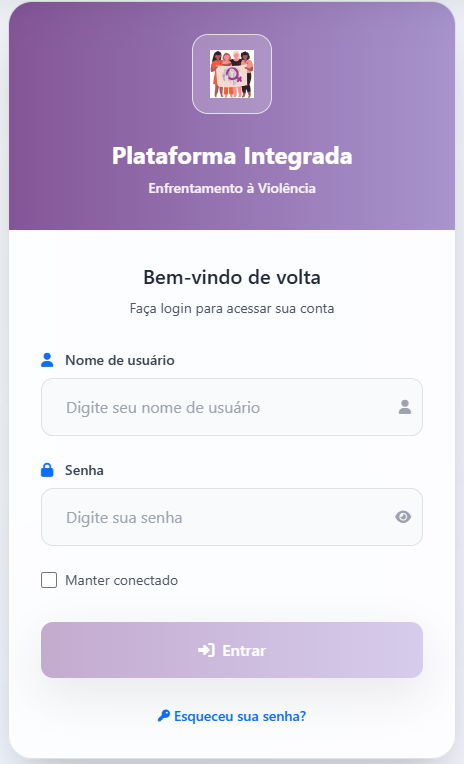
\includegraphics[scale=0.5]{figure/login.png}}
    \subfigure[Página aberta, estilo one-page.\label{fig:one-page}]{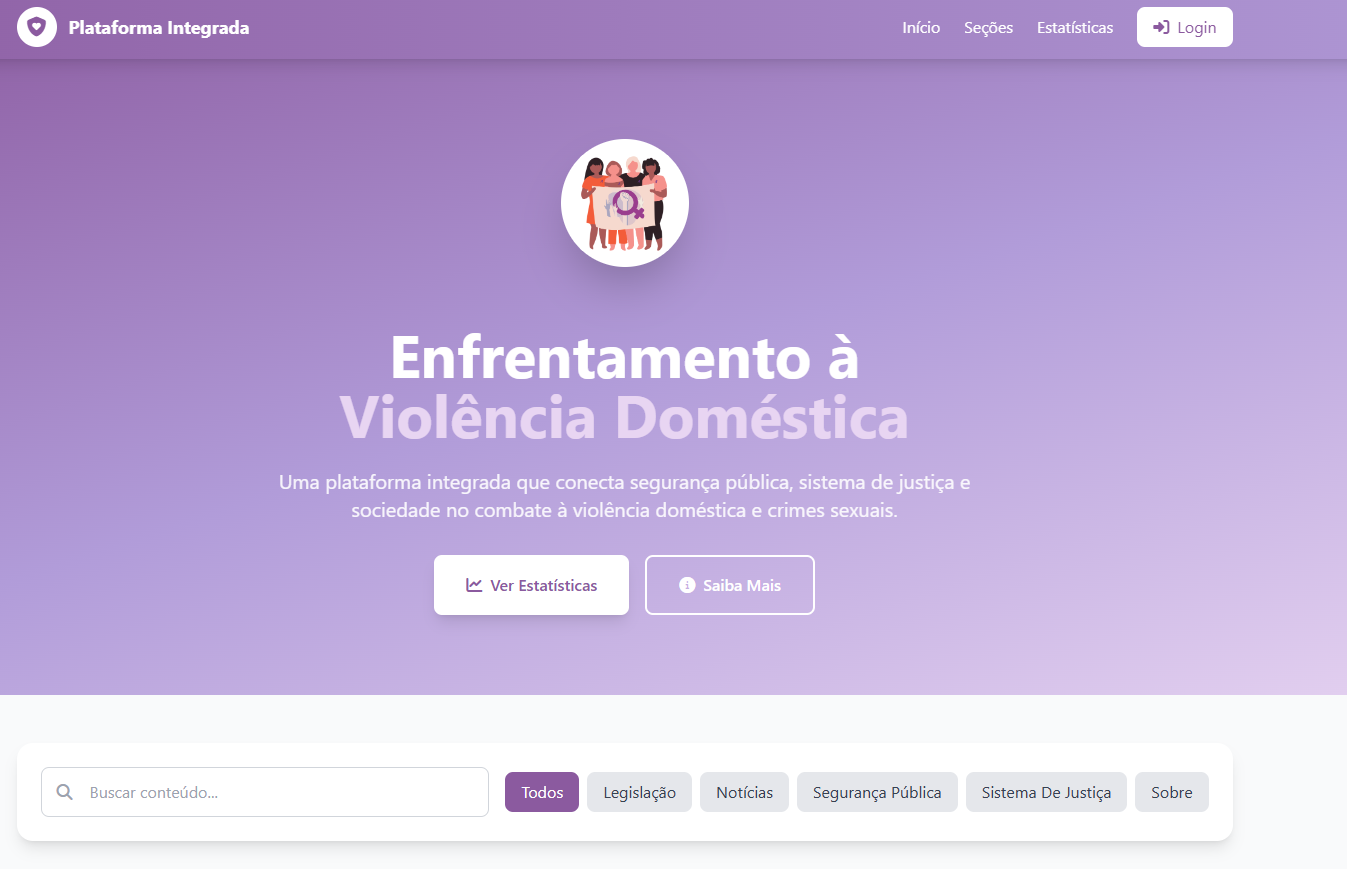
\includegraphics[scale=.2]{figure/one-page_1.png}}
    \subfigure[Página aberta, estilo one-page 1.\label{fig:one-page1}]{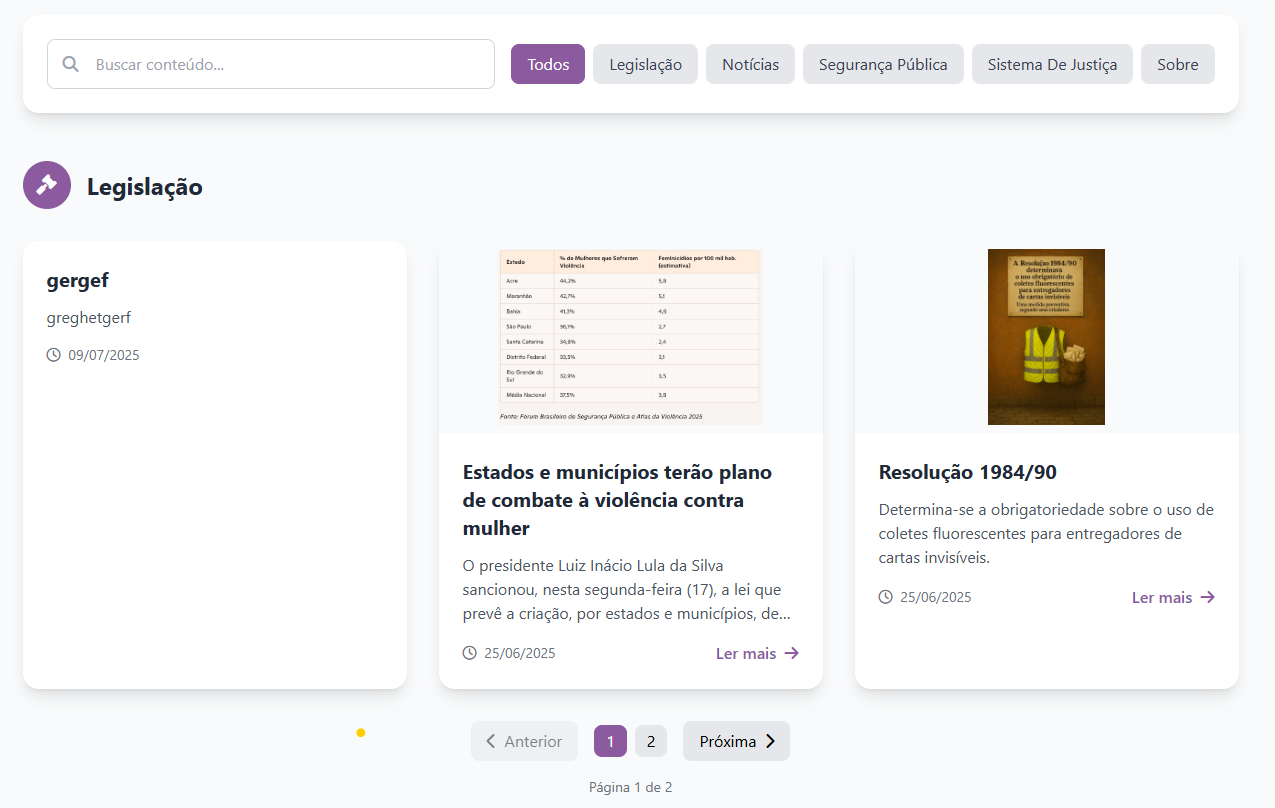
\includegraphics[scale=.2]{figure/one-page_3.png}}
    \subfigure[Página aberta, estilo one-page 2.\label{fig:one-page2}]{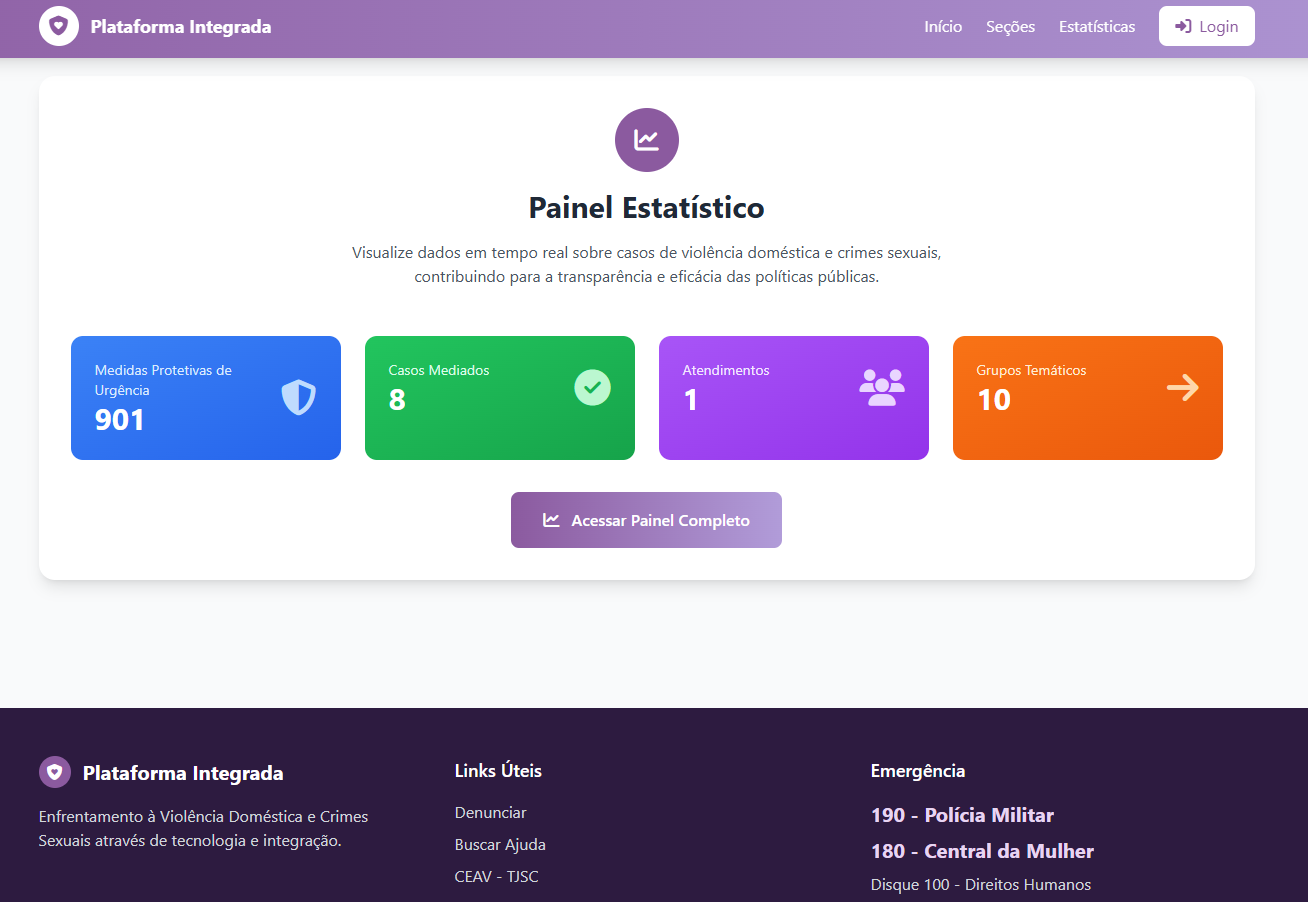
\includegraphics[scale=.2]{figure/one-page_2.png}}
    \caption{Telas da plataforma, O autor}\label{fig:telas_plataforma}
\end{figure}
\par Foi desenvolvida uma seção pública de relatórios, permitindo que portais de notícias ou entidades interessadas acessem estatísticas em tempo real. As informações apresentadas são reais e baseadas nos registros da plataforma, mas tratadas com rigor técnico para garantir o anonimato das vítimas e envolvidos. As localizações exibidas são referenciadas a centros comunitários ou órgãos públicos de cada bairro, evitando a identificação direta dos locais de ocorrência.

\begin{figure}[H]
    \center
    \subfigure[Gráfico da Etinia e Classe Econômica.\label{fig:car_map1}]{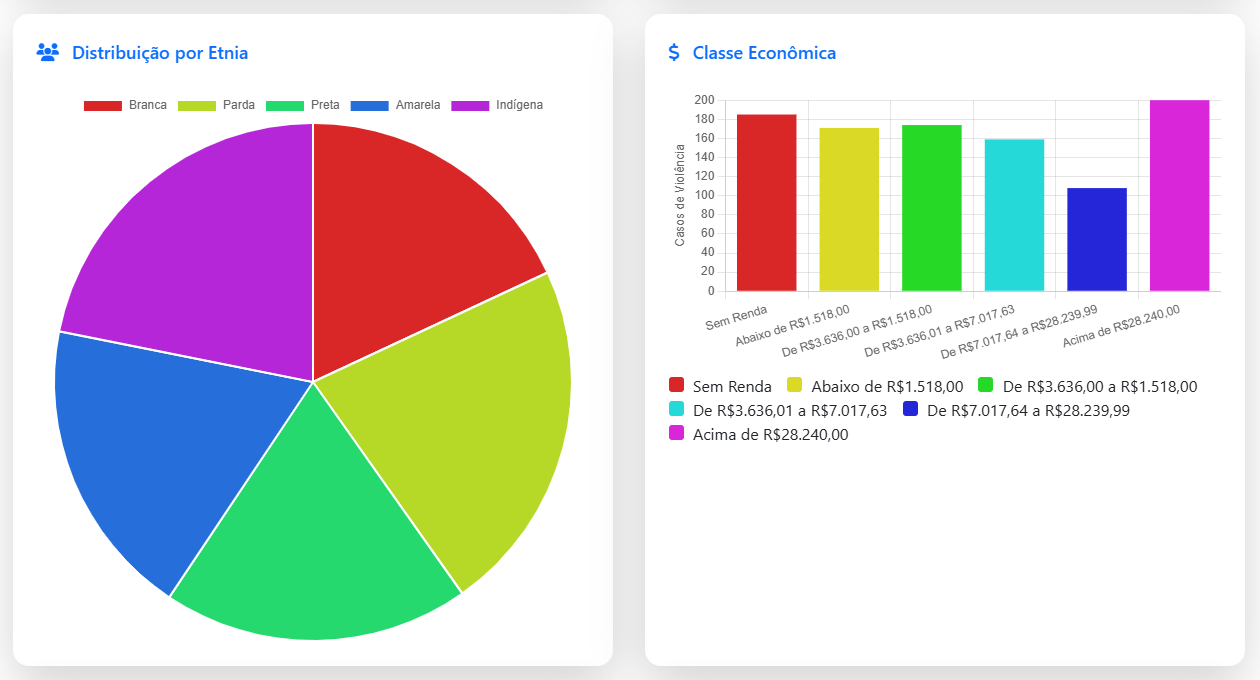
\includegraphics[scale=.2]{figure/info_3.png}}
    \subfigure[Gráfico do Grau de Instrução e Grau de Parentesco.\label{fig:car_map1}]{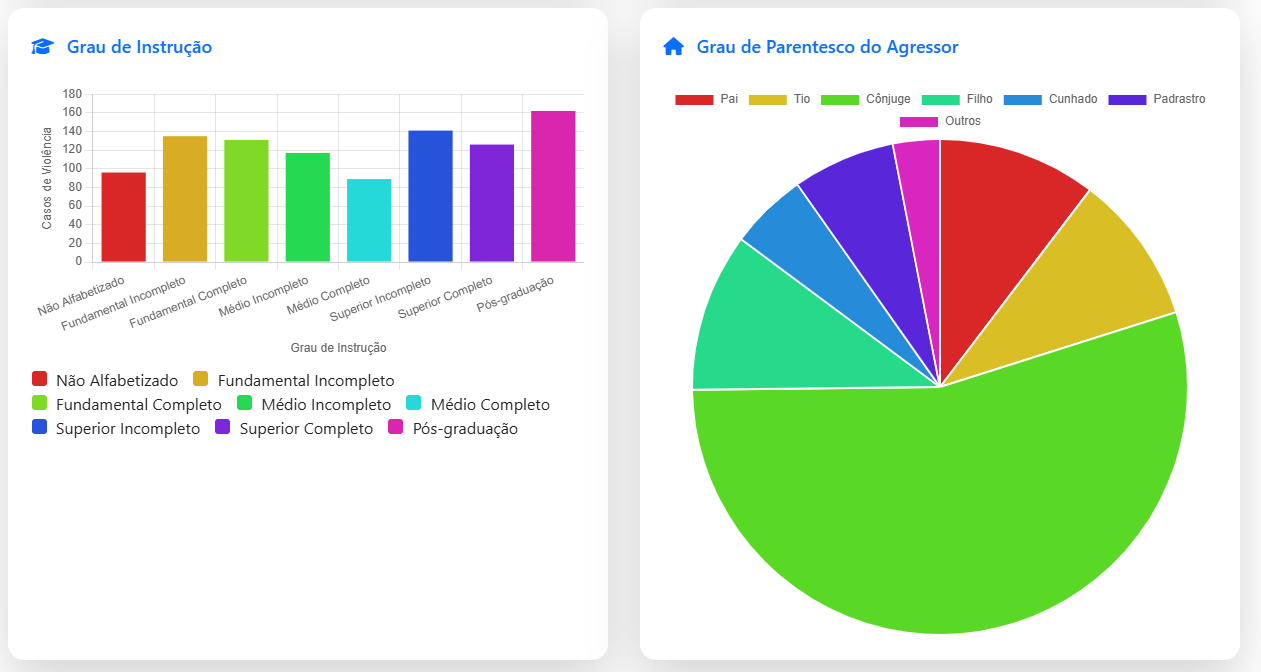
\includegraphics[scale=.2]{figure/info_1.png}}
    \subfigure[Frases Motivacionais e alguns indicadores.\label{fig:car_fras}]{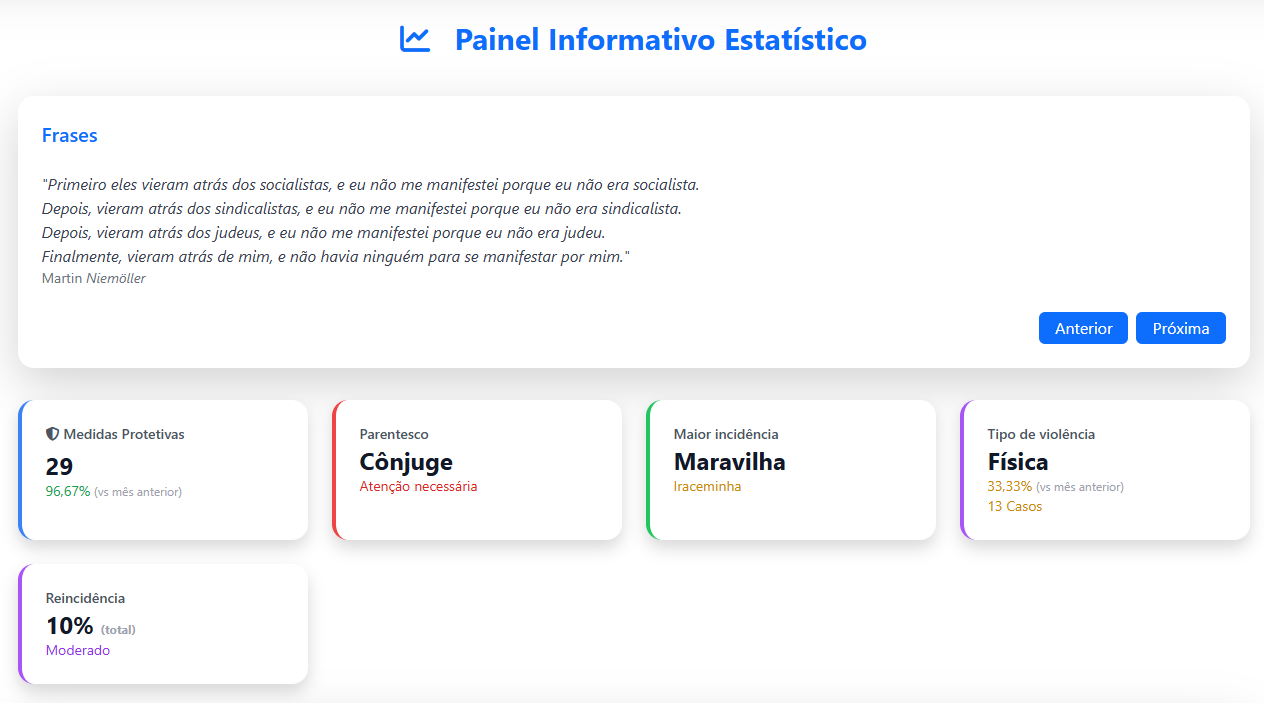
\includegraphics[scale=.4]{figure/info_2.png}}
    \subfigure[Gráfico Geográfico dos tipos de vilência.\label{fig:car_map}]{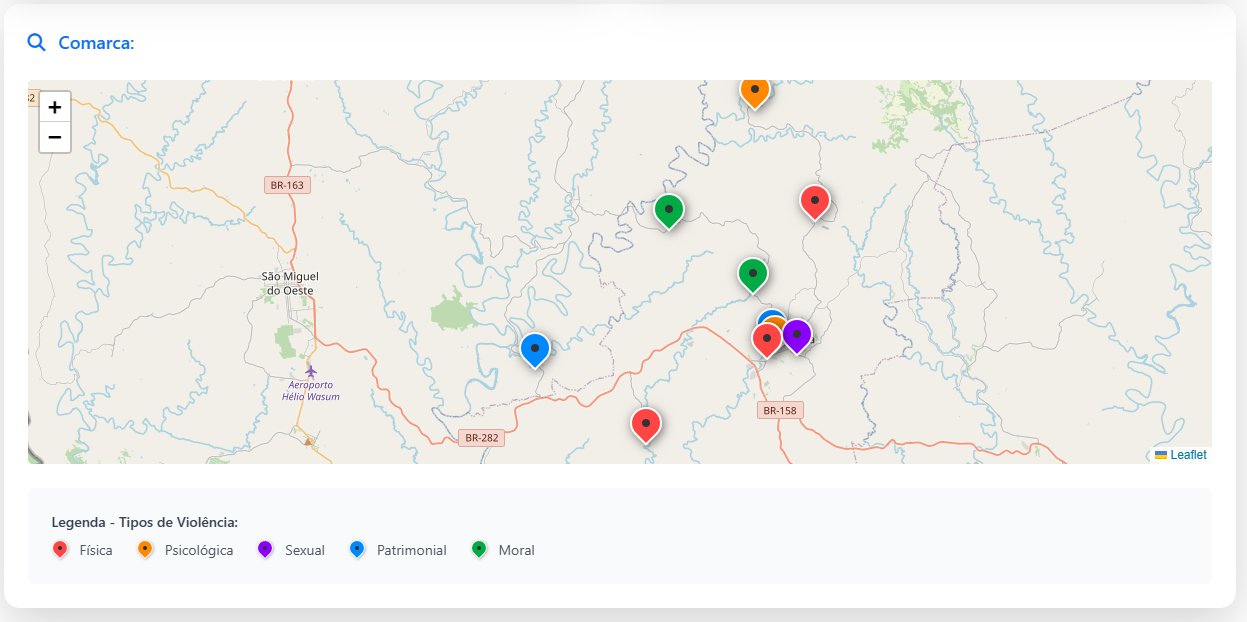
\includegraphics[scale=.5]{figure/cards_map.png}}
    \caption{Telas estatísticas, O autor}\label{fig:telas_plataforma}
\end{figure}

\par Esta sendo criada telas para cada instituição que terá acesso a plataforma e cada instituição terá determinado acesso e cada funcionalidade. Os \textit{layout} das instituições ficará a cargo de cada representante da referida em ajustar com o desenvolvedor, para usabilidade e funcionalidades de cada instituição.

\begin{figure}[H]
    \center
    \subfigure[Seleção das instituições.\label{fig:selecao_in}]{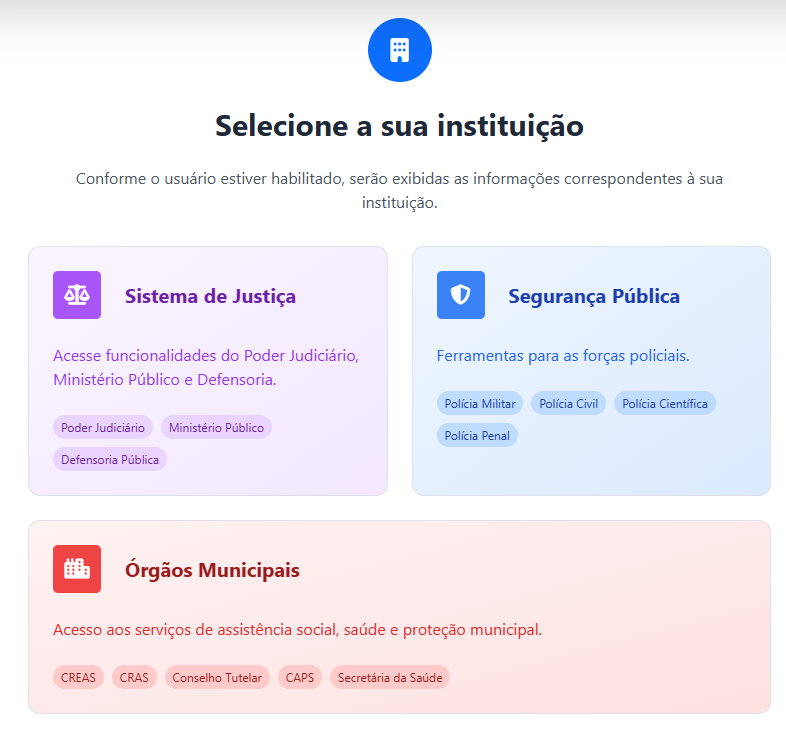
\includegraphics[scale=.3]{figure/institui.png}}
    \subfigure[Página inicial da Polícia Penal.\label{fig:home_pp}]{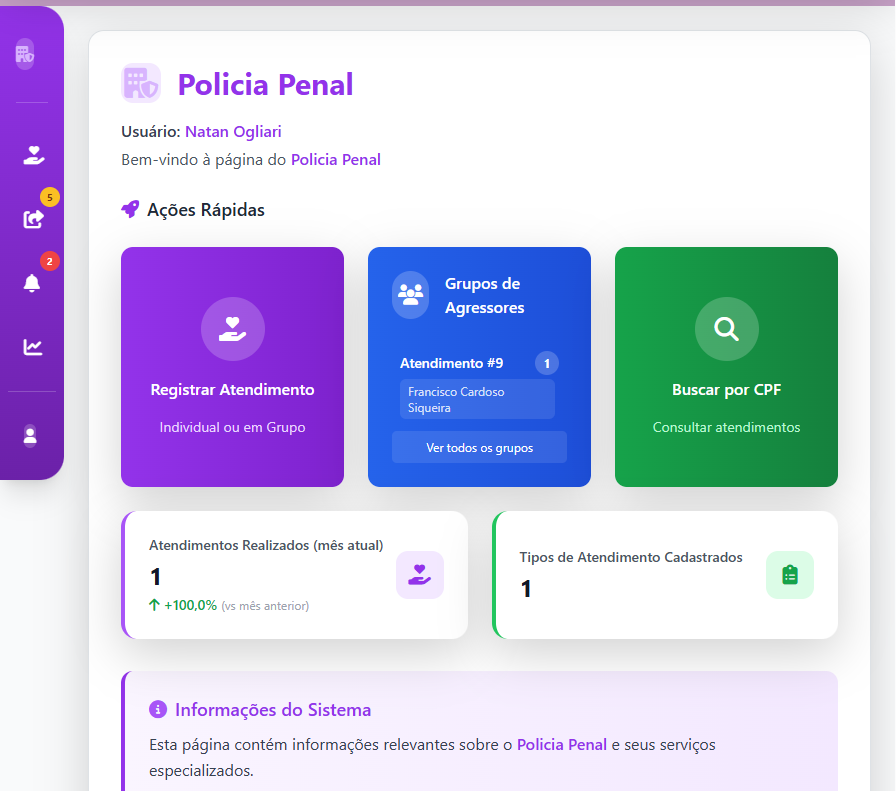
\includegraphics[scale=.3]{figure/pp_home.png}}
    \caption{Telas institucionais, O autor}\label{fig:telas_plataforma}
\end{figure}



Funcionalidades em desenvolvimento:
\begin{itemize}
    \item \textbf{Módulo de Atendimento Municipal} CRAS, CAPS, CREAS, Conselho Tutelar e Secretaria da Saúde
    \item \textbf{Módulo da segurança pública} PM, PP, PC, PCI
    \item \textbf{Integração Avançada entre Apps} Fluxos completos de encaminhamento entre órgãos
    \item \textbf{Notificações e Alertas} Sistema de notificações internas e externas
    \item \textbf{Painel Administrativo Avançado} Customização do admin para fluxos institucionais
    \item \textbf{Testes Automatizados} Cobertura de testes unitários e de integração
    \item \textbf{Aprimoramento de Relatórios} Novos filtros, exportação de dados, relatórios customizados por perfil
    \item Implantação em ambiente de produção e automação de deploy na plataforma \textit{Hostinger}
\end{itemize}


Funcionalidades Pendentes:
\begin{itemize}
    \item Integração com sistemas externos (e-eproc, MP, Defensoria, SISP)
    \item Documentação Técnica Detalhada (Swagger/OpenAPI)
    \item Aprimoramento de UX/UI para acessibilidade
    
    \item Aprimoramento de Segurança, Auditoria de logs, permissões granulares, autenticação de dois fatores
\end{itemize}

\subsection{Assistente virtual com IA}

\par A assistente virtual com inteligência artificial será uma das funcionalidade do projeto, permitindo interações mais naturais e eficientes entre os usuários e a plataforma. Utilizando técnicas de processamento de linguagem natural (PLN) e aprendizado de máquina, o assistente será capaz de compreender e responder a perguntas, fornecer orientações e realizar tarefas automatizadas.
\par Implementado e testado alguns modelos de linguagem com Ollama, algumas figuras de desempenho e respostas obtidas. Frisa-se que, alguns modelos detem de um elevado tempo de respostas isso é devido a restrição de \textit{hardware}.


\begin{figure}[H]
    \center
    \subfigure[Perguntado para a IA.\label{fig:selecao_in}]{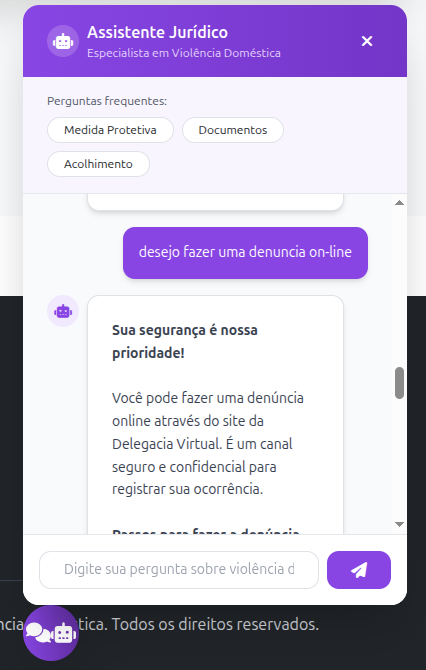
\includegraphics[scale=.3]{figure/IA_1/pergunta.png}}
    \subfigure[Resposta final da IA.\label{fig:selecao_in}]{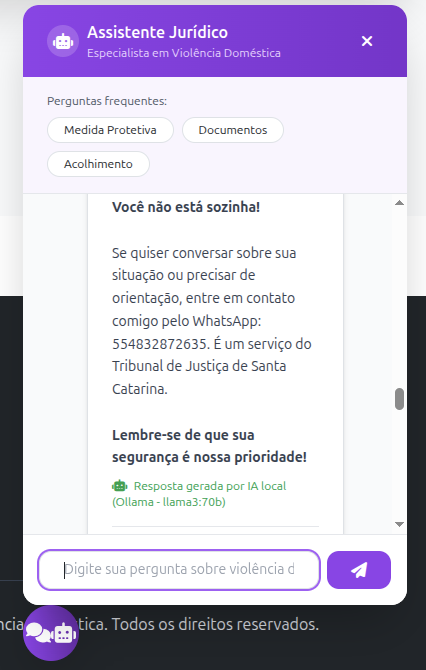
\includegraphics[scale=.3]{figure/IA_1/final_resposta.png}}
    \subfigure[Tempo para resposta.\label{fig:home_pp}]{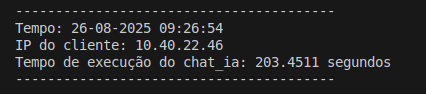
\includegraphics[scale=.3]{figure/IA_1/tempo.png}}
    \caption{Modelo llama3:70b, O autor}\label{fig:modelos_ia}
\end{figure}



\begin{algorithm}[H]
     \KwIn{Gostaria de informar que estou sofrendo, e desejo fazer uma denuncia on line. nao sei fazer a denuncia vou passar os dados e voce faz para eu.} \

    \KwResult{ \\ \textbf{Olá, querida!} \\
    Sinto muito que você esteja passando por essa situação difícil. Eu estou aqui para ajudá-la de qualquer forma possível. \\
    Antes de começar, é importante que você saiba que sua segurança é a minha prioridade. Se você se sentir ameaçada ou em perigo imediato, \textbf{por favor, ligue para o 180 (Central de Atendimento à Mulher) ou 190 (Polícia)}. Eles estarão lá para ajudá-la. \\
    Agora, sobre a denúncia on-line. Eu não posso fazer a denúncia por você, mas posso orientá-la passo a passo. Você pode acessar o site da Delegacia Virtual () e seguir as instruções. \\

    Para começar, você precisará fornecer algumas informações básicas sobre si mesma e sobre o caso de violência doméstica que está enfrentando. Isso inclui: \\

    • Seu nome e contato; \\

    • Detalhes sobre a violência sofrida (data, hora, local, etc.); \\

    • Informações sobre o agressor (nome, idade, endereço, etc.). \\

    É importante que você seja honesta e detalhista ao fornecer essas informações. Elas serão usadas para ajudá-la a obter medidas protetivas e justiça.\\


    Se você precisar de ajuda ou tiver alguma dúvida durante o processo, \textbf{por favor, entre em contato comigo pelo WhatsApp (554832872635)}. Estarei aqui para apoiá-la.\\


    Lembre-se de que você não está sozinha e que há pessoas dispostas a \\
    \texttt{ Resposta gerada por IA local (Ollama - llama3:70b)} \\
     Emergência: 190 | Central da Mulher: 180
    }

    \caption{Interação com o Modelo llama3:70b, tempo de resposta: 224.82 [s]}
   {\fontsize{10pt}{\baselineskip}\selectfont
   Fonte: O autor (2025)}

\end{algorithm}

\par A indagação ao modelo de inteligência artificial necessita para que o chatbot não crie ações que não estejam previstas. Indagou-se a possibilidade de que o chatbot realizasse uma denúncia on line, o modelo respondeu que não poderia fazer a denúncia, mas que poderia orientar a vítima a como fazer. Ressalta-se que o modelo não tem acesso a internet, e todas as respostas são geradas localmente. Ressalto que o tempo de resposta foi de \textbf{224.82 segundos}.

\section{Conclusão}

\par O projeto PIEVDCS encontra-se em estágio intermediário de desenvolvimento, com cerca de 30\% das funcionalidades previstas já implementadas. Entre os avanços, destacam-se a estrutura básica da aplicação, os modelos de dados principais, a interface inicial e os primeiros dashboards de visualização.

\par No momento, o foco está na construção dos fluxos de integração entre os órgãos, aprimoramento de velocidades nas consultas, testes e customizações de acordo com os perfis institucionais.

\par Por se tratar de um sistema que será utilizado por múltiplas instituições, sua conclusão depende da validação progressiva por parte dos usuários finais — como operadores do sistema, representantes da segurança pública, órgãos do Judiciário e Órgãos Municipais. A metodologia adotada é o Scrum, com entregas em sprints iterativos. No entanto, \textbf{não há um prazo final fixo para a entrega}, sem extrapolar o período da prestação de contas-, já que cada etapa é condicionada à disponibilidade para reuniões, testes e aprovação por parte dos \textit{stakeholders}\footnote{No contexto do desenvolvimento de sistemas, \textit{stakeholders} são todas as pessoas, grupos ou organizações que têm interesse direto ou indireto no projeto, incluindo usuários finais, clientes, desenvolvedores, patrocinadores, gestores e demais partes envolvidas no processo de criação, aprovação e uso do sistema.} (Pessoas Interresadas).

\par No tocante à assistente virtual com inteligência artificial, foram realizados testes iniciais com modelos de linguagem de grande escala (LLMs) utilizando a plataforma Ollama. Embora os resultados sejam promissores, a integração completa dessa funcionalidade na plataforma principal ainda está em fase de planejamento e desenvolvimento.

\par Este projeto é um \textbf{projeto piloto}, desenvolvido para testar a plataforma em um ambiente controlado e obter feedback prático das instituições envolvidas. Essa etapa inicial é fundamental para ajustar funcionalidades, identificar melhorias e garantir que a solução atenda efetivamente às demandas antes de uma possível expansão para outras regiões.

\par Além de seu impacto direto no enfrentamento à violência de gênero, o projeto promove inclusão e ressocialização, ao contar com a atuação técnica de um reeducando em ambiente supervisionado. A proposta comprova o potencial transformador da tecnologia aliada à reintegração social.
